\documentclass{article}
\usepackage{graphicx} % Required for inserting images
\usepackage{tikz}
\usepackage{amsmath}
\usepackage{pgfplots}
\usepackage{siunitx}

\title{Buck Converter Conduction Losses}
\author{Andrew Meares}
\date{March 2025}

\begin{document}

\maketitle

\section{Introduction}
In this paper, we derive equations for buck converter conduction losses for both FETs and diodes.  These waveforms and equations apply to continuous mode operation.

\begin{center}
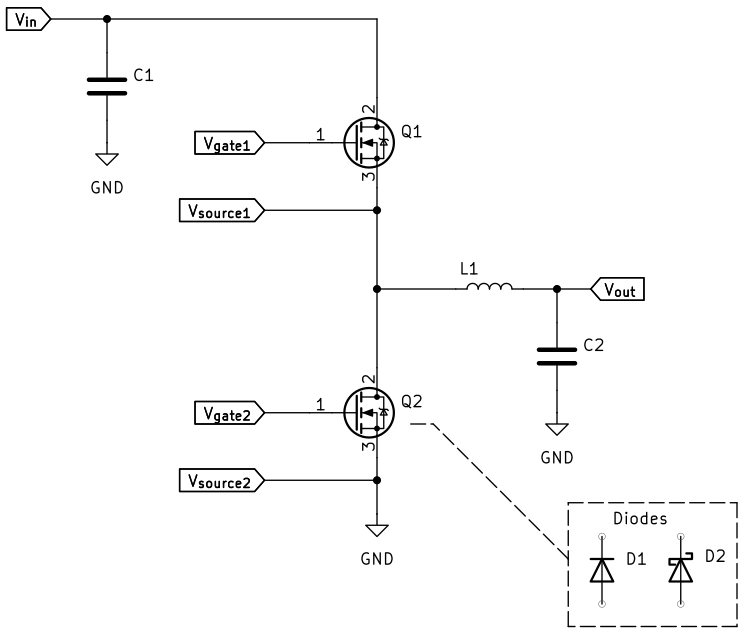
\includegraphics[width=0.5\linewidth]{buck1.png}
\end{center}

\section{Waveforms}
The waveform for the output current of a buck converter in continuous mode at equilibrium is shown below.

\begin{center}
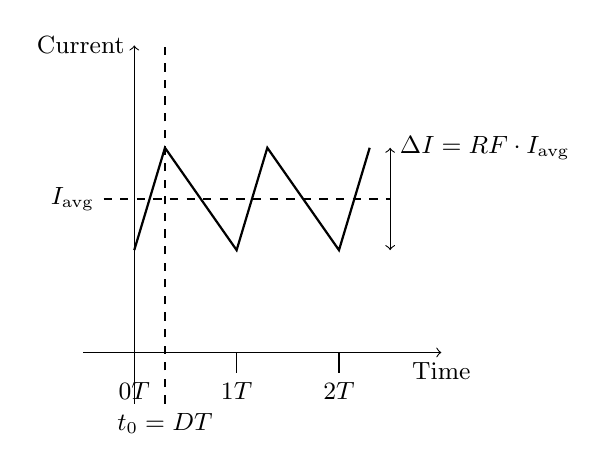
\begin{tikzpicture}[scale=1.3]
    % Axis
    \draw[->] (-0.5,0) -- (3,0) node[anchor=north] {\small Time};
    \draw[->] (0,-0.5) -- (0,3) node[anchor=east] {\small Current};
    
    % Labels for periods
    \foreach \x in {0,1,2} {
        \draw (\x,0) -- (\x,-0.2) node[anchor=north] {\small $\x T$};
    }

    % Duty cycle t0 labeled as t0 = DT
    \draw[dashed] (0.3,-0.5) -- (0.3,3);
    \node[anchor=north] at (0.3,-0.5) {\small $t_0 = D T$};

    % Iout waveform
    \draw[thick] 
        (0,1) -- (0.3,2)
        -- (1,1)
        -- (1.3,2)
        -- (2,1)
        -- (2.3,2);

    % Label for I_avg in the middle of waveform
    \draw[dashed] (-0.3,1.5) -- (2.5,1.5);
    \node[left] at (-0.3,1.5) {\small $I_{\text{avg}}$};

    % Label for RF (ripple factor)
    \draw[<->] (2.5,1) -- (2.5,2);
    \node[right] at (2.5,2) {\small $\Delta I = RF \cdot I_{\text{avg}}$};

\end{tikzpicture}
\end{center}



The waveform for a continuous mode buck converter high side switch is a repeating pulse of current as depicted below.  The slope of the triangle wave is set by the inductance at that operating point. \\

\begin{center}
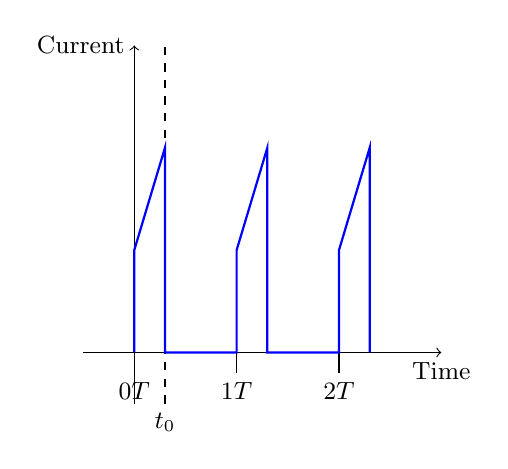
\begin{tikzpicture}[scale=1.3]
    % Axis
    \draw[->] (-0.5,0) -- (3,0) node[anchor=north] {\small Time};
    \draw[->] (0,-0.5) -- (0,3) node[anchor=east] {\small Current};
    
    % Labels for periods
    \foreach \x in {0,1,2} {
        \draw (\x,0) -- (\x,-0.2) node[anchor=north] {\small $\x T$};
    }

    % Duty cycle t0
    \draw[dashed] (0.3,-0.5) -- (0.3,3);
    \node[anchor=north] at (0.3,-0.5) {\small $t_0$};

    % Input current waveform
    \draw[thick, blue] 
        (0,0) -- (0,1)
        -- (0.3,2)
        -- (0.3,0)
        -- (1,0)
        -- (1,1)
        -- (1.3,2)
        -- (1.3,0)
        -- (2,0)
        -- (2,1)
        -- (2.3,2)
        -- (2.3,0);     

\end{tikzpicture}
\end{center}

For a converter with a theoretical 100\% efficiency, the input and output power are equal.  The average pulse height is the same as the average output current due to Kirchoff's current law.  This means for a 50A converter, the input current is in 50A pulses at the higher Vin with a duty cycle, $D = \frac{V_o}{V_i}$ and a ripple factor, $RF = \frac{\Delta I}{I_\text{avg}}$.

The rectifier sees a falling current with the same average.

\begin{center}
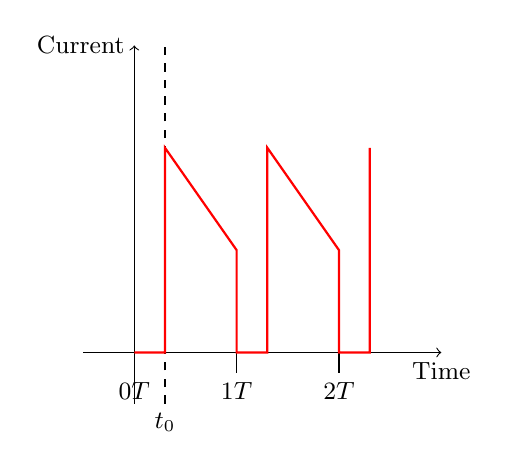
\begin{tikzpicture}[scale=1.3]
    % Axis
    \draw[->] (-0.5,0) -- (3,0) node[anchor=north] {\small Time};
    \draw[->] (0,-0.5) -- (0,3) node[anchor=east] {\small Current};

    % Labels for periods
    \foreach \x in {0,1,2} {
        \draw (\x,0) -- (\x,-0.2) node[anchor=north] {\small $\x T$};
    }

    % Duty cycle t0
    \draw[dashed] (0.3,-0.5) -- (0.3,3);
    \node[anchor=north] at (0.3,-0.5) {\small $t_0$};

    % Rectifier current waveform (falling slope)
    \draw[thick, red] 
        (0,0) -- (0.3,0)
        -- (0.3,2)
        -- (1,1)
        -- (1,0)
        -- (1.3,0)
        -- (1.3,2)
        -- (2,1)
        -- (2,0)
        -- (2.3,0)
        -- (2.3,2);

\end{tikzpicture}
\end{center}

\section{Rectifier Derivation}

Assuming the rectifier is a diode with a constant forward voltage, the power in the diode is simply:

\begin{equation}
P_\text{diode} = (1-D) V_\text{f} I_\text{avg}
\end{equation}

If the diode is replaced with a FET, the conduction losses are harder to calculate.  Start with the power loss equation for a resistive element:

\[
P_\text{FET} = \frac{1}{T} \int_{0}^{T} R_\text{dson} i^2(t) \, dt
\]

We split the integral:

\[
P_\text{FET} = \frac{1}{T} \left[\int_{0}^{t_0} R_\text{dson} i^2(t) \, dt + \int_{t_0}^{T} R_\text{dson} i^2(t) \, dt \right]
\]

Since \( i(t) = 0 \) for \( 0 \leq t < t_0 \), this simplifies to:

\[
P_\text{FET} = \frac{1}{T} \left[ 0 + \int_{t_0}^{T} R_\text{dson} \left( I_\text{avg} \left( 1+\frac{RF}{2} \right) - \frac{RF I_\text{avg}}{T-t_0}(t-t_0) \right)^2 \, dt \right]
\]

Using \( D = \frac{t_0}{T} \), we rewrite:

\[
P_\text{FET} = \frac{R_\text{dson}}{T} \int_{t_0}^{T} \left( I_\text{avg} \left(1+\frac{RF}{2} \right) - \frac{RF I_\text{avg}}{(1-D)T}(t-t_0) \right)^2 \, dt
\]

Factor out \( I_\text{avg}^2 \):

\[
P_\text{FET} = \frac{R_\text{dson} I_\text{avg}^2}{T} \int_{t_0}^{T} \left( \left(1+\frac{RF}{2} \right) - \frac{RF}{(1-D)T}(t-t_0) \right)^2 \, dt
\]

Expanding the square:

\[
\left( (1+\frac{RF}{2})-\frac{RF}{(1-D)T}(t-t_0) \right)^2
\]

\[
= \left(1 + \frac{RF}{2} \right)^2 - 2 \left(1 + \frac{RF}{2} \right) \frac{RF}{(1-D)T} (t-t_0) + \left( \frac{RF}{(1-D)T} (t-t_0) \right)^2
\]

Splitting the integral:

%\[
%P_\text{FET} = \frac{R I_\text{avg}^2}{T} \left[ (1+\frac{RF}{2})^2 \int_{t_0}^{T} dt - %2(1+\frac{RF}{2}) \frac{RF}{(1-D)T} \int_{t_0}^{T} (t-t_0) dt + \left( \frac{RF}{(1-D)T} %\right)^2 \int_{t_0}^{T} (t-t_0)^2 dt \right]
%\]

\[
P_\text{FET} = \frac{R_\text{dson} I_\text{avg}^2}{T} \Bigg[
(1+\frac{RF}{2})^2 \int_{t_0}^{T} dt 
- 2(1+\frac{RF}{2}) \frac{RF}{(1-D)T} \int_{t_0}^{T} (t-t_0) dt 
\]
\[
+ \left( \frac{RF}{(1-D)T} \right)^2 \int_{t_0}^{T} (t-t_0)^2 dt 
\Bigg]
\]

Computing the integrals:

\[
\int_{t_0}^{T} dt = (1-D)T
\]

\[
\int_{t_0}^{T} (t-t_0) dt = \frac{(1-D)^2T^2}{2}
\]

\[
\int_{t_0}^{T} (t-t_0)^2 dt = \frac{(1-D)^3T^3}{3}
\]

Substituting back:

%\[
%P_\text{FET} = \frac{R I_\text{avg}^2}{T} \left[ (1+\frac{RF}{2})^2 (1-D)T - 2(1+\frac{RF}%{2}) \frac{RF}{(1-D)T} \cdot \frac{(1-D)^2T^2}{2} + \left(\frac{RF}{(1-D)T} \right)^2 \cdot %\frac{(1-D)^3T^3}{3} \right]
%\]

\[
P_\text{FET} = \frac{R_\text{dson} I_\text{avg}^2}{T} \Bigg[
(1+\frac{RF}{2})^2 (1-D)T 
- 2(1+\frac{RF}{2}) \frac{RF}{(1-D)T} \cdot \frac{(1-D)^2T^2}{2} 
\]
\[
+ \left(\frac{RF}{(1-D)T} \right)^2 \cdot \frac{(1-D)^3T^3}{3} 
\Bigg]
\]

Canceling \(T\):

\[
P_\text{FET} = R_\text{dson} I_\text{avg}^2 \left[ (1+\frac{RF}{2})^2 (1-D) - (1+\frac{RF}{2})RF (1-D) + \frac{RF^2 (1-D)}{3} \right]
\]

Factoring out \( (1-D) \):

\begin{equation}
P_\text{FET} = R_\text{dson} I_\text{avg}^2 (1-D) \left[ (1+\frac{RF}{2})^2 - (1+\frac{RF}{2})RF + \frac{RF^2}{3} \right]
\end{equation}

Here is a plot of the part of the equation depending on ripple factor.

\begin{center}
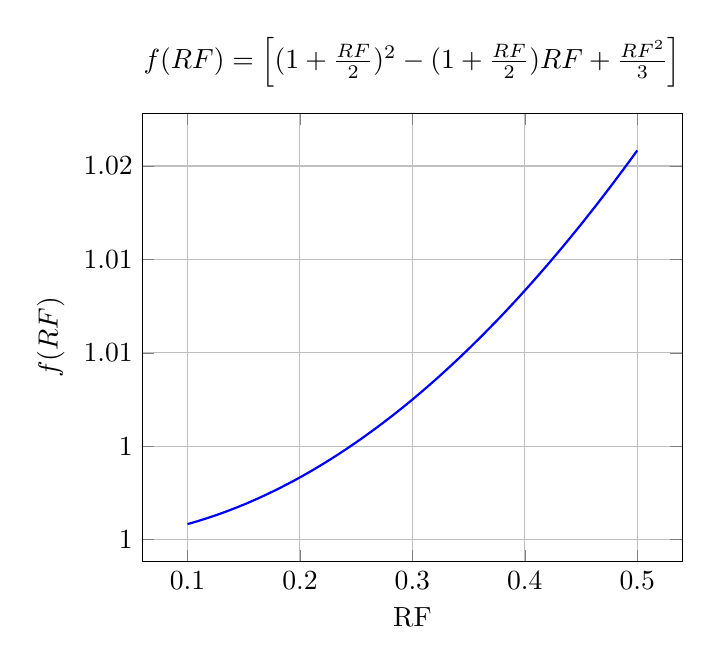
\begin{tikzpicture}
    \begin{axis}[
        xlabel={RF},
        ylabel={$f(RF)$},
        title={$f(RF) = \left[ (1+\frac{RF}{2})^2 - (1+\frac{RF}{2})RF + \frac{RF^2}{3} \right]$},
        domain=0.1:0.5,
        samples=100,
        grid=major
    ]
        \addplot [
            thick,
            blue
        ] 
        { (1 + x/2)^2 - (1 + x/2)*x + x^2/3 };
    \end{axis}
\end{tikzpicture}
\end{center}

The surprise here is that the effect of ripple factor is only a few percent.\\

Here is the simplified result:
\begin{equation}
P_\text{FET} \approx R_\text{dson} I_\text{avg}^2 (1-D)
\end{equation}

The conduction losses of the FET and the diode will equal when:
\[
R_\text{dson} I_\text{avg}^2 (1-D) = (1-D) V_\text{f} I_\text{avg}
\]

\[
R_\text{dson} I_\text{avg}^2 = V_\text{f} I_\text{avg}
\]

\begin{equation}
\frac{V_\text{f}}{R_\text{dson}} = I_\text{avg}
\end{equation}

\section{Temperature Estimate Examples}
A high input voltage might reasonably yield a duty cycle of \num{0.2}.
Consider that the FET has a \qty{0.5}{\celsius} better junction to case coefficient.
Assume perhaps that the heatsink to junction total is \qty{7}{\celsius\per\watt} for the diode and \qty{6.5}{\celsius\per\watt} for the FET.
It is clear that both a single TO-220 diode or FET get too hot.
Assume the diode $V_\text{f}$ is \qty{0.65}{\volt} and the FET $R_\text{dson}$ is \qty{0.013}{\ohm}.  I chose these values because the conduction losses are equal at \qty{26}{\watt}.

\[
T_\text{diode} = (\num{1}-\num{0.2}) (\qty{0.65}{\volt}) (\qty{50}{\ampere}) (\qty{7}{\celsius\per\watt}) + \qty{25}{\celsius} = \qty{182}{\celsius}
\]

\[
T_\text{FET} = (1-0.2) (\qty{0.013}{\ohm}) (\qty{50}{\ampere})^2 (\qty{6.5}{\celsius\per\watt}) + \qty{25}{\celsius} = \qty{169}{\celsius}
\]

Now consider two parallel diodes or FETs.

\[
T_\text{diode} = \frac{1}{2}(\num{1}-\num{0.2}) (\qty{0.65}{\volt}) (\qty{50}{\ampere}) (\qty{7}{\celsius\per\watt}) + \qty{25}{\celsius} = \qty{116}{\celsius}
\]

\[
T_\text{FET} = \frac{1}{2}(\num{1}-\num{0.2}) (\frac{\qty{0.013}{\ohm}}{2}) (\qty{50}{\ampere})^2 (\qty{6.5}{\celsius\per\watt}) + \qty{25}{\celsius} = \qty{67}{\celsius}
\]

Total power lost differs now with our choice of two devices.  The FETs now dissipate half the power of the diodes.

\[
P_\text{diode} = \num{0.8} (\qty{0.65}{\volt}) (\qty{50}{\ampere}) = \qty{26}{\watt}
\]

\[
P_\text{FET} = \num{0.8} (\frac{\qty{0.013}{\ohm}}{2}) (\qty{50}{\ampere})^2 = \qty{13}{\watt}
\]

Note FETs will have more switching losses than diodes and more devices will similarly multiply those losses.  Switching losses will need some addressing if we are to properly compare the two technologies.

\section{High Side Losses}
So, now we painstakingly derive the high side losses? \\

If the pattern follows from the bottom side rectifier, you eventually simplify to:
\begin{equation}
P_\text{FET} = D R_\text{dson} I_\text{avg}^2 f(RF)
\end{equation}

Where $f(RF) \approx 1$ is some function of the ripple factor.  I argue that the power measurement behaves the same if we flip time such that:

\[
t \to T - t.
\]

That means:
\begin{itemize}
    \item The inductor current waveform does not change in shape.
    \item The power integral structure must be the same.
\end{itemize}

\begin{center}
\begin{minipage}{0.4\textwidth}
\centering
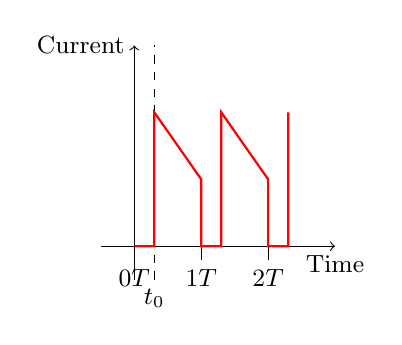
\begin{tikzpicture}[scale=0.85]
    % Axis
    \draw[->] (-0.5,0) -- (3,0) node[anchor=north] {\small Time};
    \draw[->] (0,-0.5) -- (0,3) node[anchor=east] {\small Current};

    % Labels for periods
    \foreach \x in {0,1,2} {
        \draw (\x,0) -- (\x,-0.2) node[anchor=north] {\small $\x T$};
    }

    % Duty cycle t0
    \draw[dashed] (0.3,-0.5) -- (0.3,3);
    \node[anchor=north] at (0.3,-0.5) {\small $t_0$};

    % Rectifier current waveform (falling slope)
    \draw[thick, red] 
        (0,0) -- (0.3,0)
        -- (0.3,2)
        -- (1,1)
        -- (1,0)
        -- (1.3,0)
        -- (1.3,2)
        -- (2,1)
        -- (2,0)
        -- (2.3,0)
        -- (2.3,2);
\end{tikzpicture}
\end{minipage}
\hfill
\begin{minipage}{0.15\textwidth}
\centering
\vspace{1.5cm}
\large{$t \rightarrow T - t$}
\end{minipage}
\hfill
\begin{minipage}{0.4\textwidth}
\centering
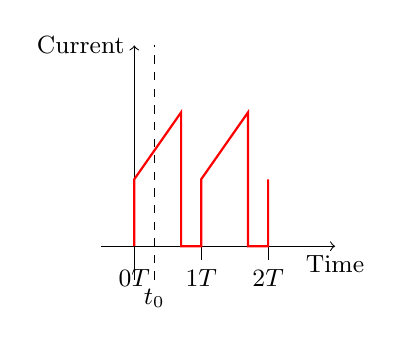
\begin{tikzpicture}[scale=0.85]
    % Axis
    \draw[->] (-0.5,0) -- (3,0) node[anchor=north] {\small Time};
    \draw[->] (0,-0.5) -- (0,3) node[anchor=east] {\small Current};

    % Labels for periods
    \foreach \x in {0,1,2} {
        \draw (\x,0) -- (\x,-0.2) node[anchor=north] {\small $\x T$};
    }

    % Duty cycle t0
    \draw[dashed] (0.3,-0.5) -- (0.3,3);
    \node[anchor=north] at (0.3,-0.5) {\small $t_0$};

    % Rectifier current waveform (rising slope)
    \draw[thick, red] 
        (0,0) -- (0,1)
        -- (0.7,2)
        -- (0.7,0)
        -- (1,0)
        -- (1,1)
        -- (1.7,2)
        -- (1.7,0)
        -- (2,0)
        -- (2,1);
\end{tikzpicture}
\end{minipage}
\end{center}

Based on this time-reversal principal, the unknown function $f(RF)$ is exactly the same for the high and low side FETs and is:

\begin{equation}
f(RF) = \left[ (1+\frac{RF}{2})^2 - (1+\frac{RF}{2})RF + \frac{RF^2}{3} \right]
\end{equation}

Finally, the result is similar to before:

\begin{equation}
P_\text{FET} \approx D R_\text{dson} I_\text{avg}^2
\end{equation}

\section{Conclusion}
Our estimates here are based on waveforms and a simple unchanging resistance or forward voltage.  In practice, those values are at least functions of temperature and/or current.  One approach here is repeated calculation to converge on the correct solution based on datasheet charts.

Conduction losses are only one portion of the total losses in a switching power converter.
Switching losses are a concern, especially with FETs.  A quick estimate would be to add some fixed percentage of the conduction losses.

Furthermore, these equations only apply to continuous conduction mode buck converters, though other converters and modes may show similarities.

\end{document}
